\documentclass{article}
\usepackage{sourcesanspro}
\usepackage[letterpaper, margin=1in]{geometry}
\setlength{\parskip}{0.5em}
\setlength\parindent{0pt}
\usepackage{graphicx} % Required for inserting images
\usepackage{listings}
\usepackage{xcolor} % to access the named colour LightGray
\usepackage{tcolorbox}
\usepackage[T1]{fontenc}
\usepackage{amssymb}
\usepackage{hyperref}

\definecolor{myblue}{RGB}{0,0,255}
\hypersetup{
    linktoc=all,
    colorlinks=true,
    linkcolor=black,
    filecolor=red,
    urlcolor=myblue,
    pdftitle={PhD Confirmation Report},
    citecolor=myblue,
}

\newcommand{\cmd}[1] {{\color{teal}  #1}}
\newcommand{\ope}[1] {{\color{purple}#1}}
\newcommand{\cmt}[1] {{\color{violet}#1}}

\newcommand{\definition}[1] {
    \begin{tcolorbox}[colback=white,colframe=mygray,sharp corners=all,top=0.01cm,bottom=0.01cm,left=0.1cm]
        {\fontfamily{pcr}\selectfont #1}
    \end{tcolorbox}
}

\definecolor{mygray}{RGB}{230,230,230}
\newcommand{\code}[1] {
    \begin{tcolorbox}[colback=mygray,colframe=mygray,sharp corners=all,top=0.01cm,bottom=0.01cm,left=0.1cm]
        \small
        {\fontfamily{pcr}\selectfont
        #1
        }

    \end{tcolorbox}
}

\title{Python-CPSolver reference manual}
\author{Gonzalo Hernandez}
\date{September 2024}

\begin{document}

\maketitle

\tableofcontents
\newpage
% ----------------------------------------------------------------------------------

\section{Introduction}

Python-CPSolver is a flexible and simple tool that leverages constraint technologies to search for solutions over large data spaces. It provides all the necessary components to effectively tackle complex constraint-based problem. It is designed to implement and understand various algorithms for solving combinatorial problems, as described in the literature and adapted to constraint-solving techniques. Rather than focusing on creating a competitive tool, Python-CPSolver aims to provide a user-friendly environment for validating and developing new methods.

Keeping our core purpose in mind, Python-CPSolver [\href{https://github.com/GonzaloHernandez/python-cpsolver}{See GitHub}] comprises four essential modules: Searching, Variables, Branching, and Propagators. Each of these modules was crafted with a minimalist approach, prioritising simplicity over efficiency. For a clearer grasp of our intent, consider our overuse of Python Lists, chosen for their versatility and utility over creating specialised data structures for similar tasks.

\begin{figure}[h]
    \centering
    \noindent{\begin{minipage}{\dimexpr\textwidth-70\fboxsep-2\fboxrule\relax}
        \centering
        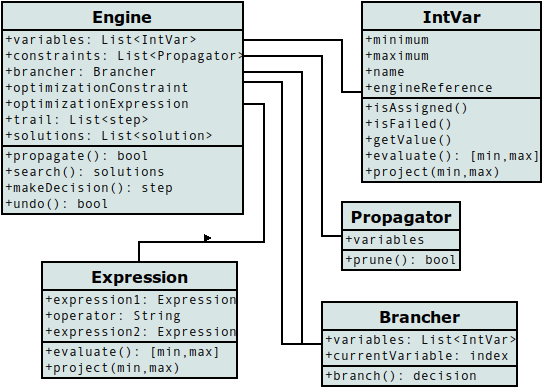
\includegraphics[width=1\linewidth]{figures/python-cpsolver-01.png}
    \end{minipage}}
    \caption{General UML for Python-CPSolver}
    \label{fig:python-cpsolver_01}
\end{figure}

Figure \ref{fig:python-cpsolver_01} provides a comprehensive overview of the inner workings of Python-CPSolver. It is implemented using Object-Oriented Programming, drawing inspiration from the structures of Gecode and Chuffed. Some identifiers of classes, attributes, and methods are borrowed from these two solvers, while other segments of the code are based on the CPFloat-Gecode project [\href{https://github.com/GonzaloHernandez/cpfloat-gecode}{See}].

At the heart of Python-CPSolver lies the Engine class, which orchestrates the search process and serves as the nexus for other classes. Within this class, we find storage for sets of variables and propagators, as well as the optimisation expression and its corresponding propagator. In the latest version (Version-Trail), this class also maintains the trail, tracking the progress of the ongoing search. Its central procedure, "search", iteratively calls upon "propagate", "makeDecision", and "undo" to navigate through the search space. An example of extending this solver by creating new propagators is shown in Figure \ref{fig:python-cpsolver_02}

\begin{figure}[ht]
    \centering
    \noindent{\begin{minipage}{\dimexpr\textwidth-70\fboxsep-2\fboxrule\relax}
        \centering
        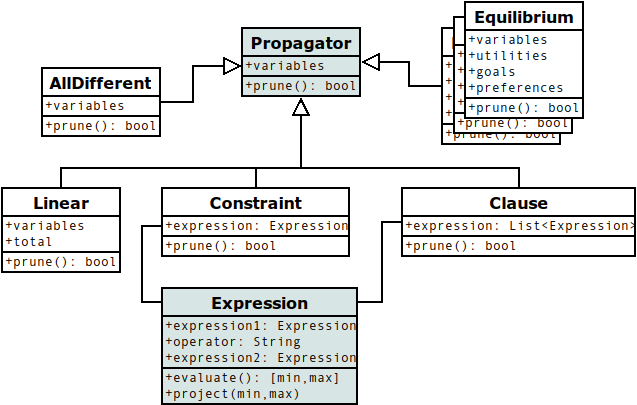
\includegraphics[width=1\linewidth]{figures/python-cpsolver-02.png}
    \end{minipage}}
    \caption{Propagators module for Python-CPSolver}
    \label{fig:python-cpsolver_02}
\end{figure}

Python-CPSolver is crafted with a commitment to simplicity while preserving the essence of Constraint technologies. Each implementation of a propagator retains a copy of the variables, either directly or through an expression. Additionally, these classes override the "prune" method, responsible for filtering and checking satisfiability.

While creating specialized propagators enhances efficiency, it is crucial to highlight the significance of the Constraint as a generic propagator. Python-CPSolver utilizes the HC4 algorithm \cite{araya:2008} to evaluate and filter mathematical expressions using Box Consistency. These expressions are represented in a tree structure through the Expression class. The algorithm operates in two phases: the first phase evaluates the expression in an upward pass, and the second phase performs filtering in a downward pass. Figure \ref{fig:hc4}, adapted from \cite{araya:2008}, illustrates these phases.

\begin{figure}[ht]
    \centering
    \noindent{\begin{minipage}{\dimexpr\textwidth-70\fboxsep-2\fboxrule\relax}
        \centering
        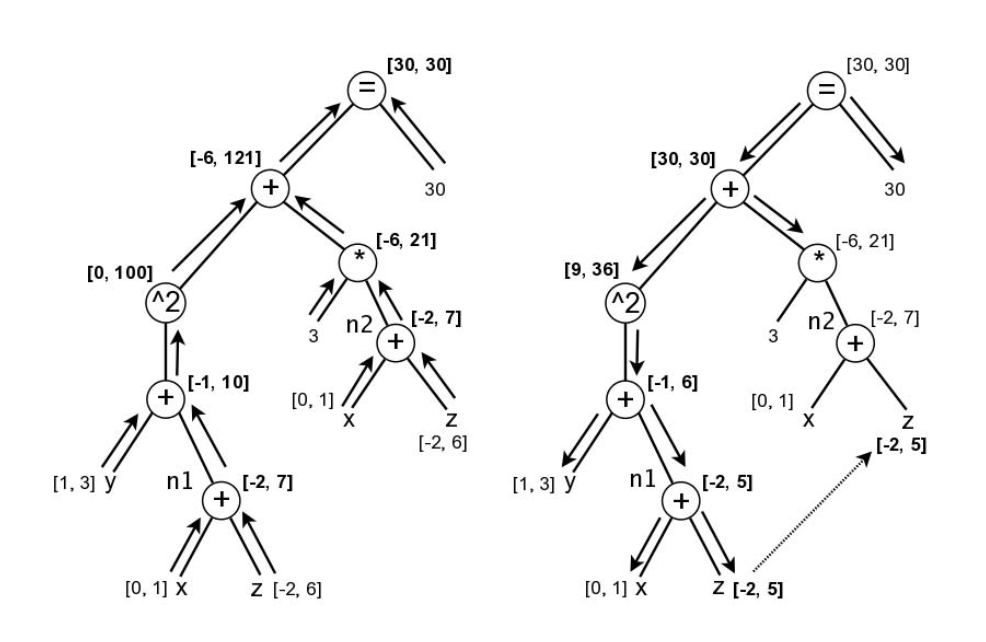
\includegraphics[width=1\linewidth]{figures/hc4.png}
    \end{minipage}}
    \noindent{\begin{minipage}{\dimexpr\textwidth-60\fboxsep-2\fboxrule\relax}
        \caption{Evaluation and narrowing in the HC4-revise algorithm. The tree represents the constraint: $(x + y + z) 2 + 3(x + z) = 30$.}
        \label{fig:hc4}
    \end{minipage}}
\end{figure}

\section{Installation}

Prerequisites: To use this software, you only need Python 3. It can be easily installed directly from the Python Package Index (PyPI) and works out of the box.

\code{pip install PythonCPSolver}

Additionally, since this software is designed for evaluating new algorithms, the source code is available on GitHub:

\href{https://github.com/GonzaloHernandez/python-cpsolver}{https://github.com/GonzaloHernandez/python-cpsolver}

\section{Playing}

\textit{CSP} $ = (X,(D_i)_{i \in X},C)$ \cite{apt:2003}

\textit{cpsolver}: \textit{CSP} $ \rightarrow \{(x_i,d_i) \mid x_i \in X, d_i \in D_i, \forall C_j \in C : C_j \textit{ is satisfied }\}$

\subsection{How to use}

Python-CPSolver consists of four core modules: engine, brancher, propagators, and variables. In most scenarios, importing the entire package is adequate for utilizing Python-CPSolver. A basic program typically includes five main sections: \\

\definition{ 
    - <package> \\
    - <decision\_variables> {\footnotesize [See section \ref{sec:variables}]}\\
    - <constraints> {\footnotesize [See section \ref{sec:constraints}]}\\
    - <seraching> {\footnotesize [See section \ref{sec:searching}]}\\
    - <output> {\footnotesize [See section \ref{sec:output}]}
}

\code{
    \cmt{\# package} \\
    \cmd{from} PythonCPSolver \cmd{import} \ope{*} \\

    \cmt{\# decision variables} \\
    x \ope{=} IntVar(1,5) \\
    y \ope{=} IntVar(3,8) \\
    z \ope{=} IntVar(1,10) \\

    \cmt{\# constraints} \\
    constraint1 \ope{=} AllDifferent([x,y,z]) \\
    constraint2 \ope{=} Constraint(x\ope{+}y \ope{==} z) \\
    
    \cmt{\# searching} \\
    engine \ope{=} Engine( [x,y,z], [constraint1,constraint2] ) \\    
    solutions \ope{=} engine.search() \\

    \cmt{\# output} \\
    \cmd{for} s \cmd{in} solutions : print( toInts(s) ) 
}

This example will show the first solution found: $(x_1=1, x_2=3, x_3=4)$.

\subsection{Variables and Expressions}\label{sec:variables}

Python-CPSolver uses a generic integer variable type with bounds $-2147483647 \leqslant x \leqslant 2147483647$, where the parameters primarily set the limits.\\

\definition{ IntVar(min:\cmd{int}, max:\cmd{int}, name:\cmd{int} ) : IntVar}

\code{
    x1 \ope{=} IntVar(1,10,"var")\\
    x2 \ope{=} IntVar(-5,4)\\
    x3 \ope{=} IntVar(3) \\
    x4 \ope{=} IntVar()
}

This example instanciates $x_1$ labeld as \textit{var}, and $x_2,x_3,x_4$ without labels, where $(1 \leqslant x_1 \leqslant 10)$, $(-5 \leqslant x_2 \leqslant 4)$, $(3 \leqslant x_3 \leqslant 2147483647)$ and $(-2147483647 \leqslant x_4 \leqslant 2147483647)$.\\

\definition{ IntVarArray(n:\cmd{int}, min:\cmd{int}, max:\cmd{int}, prefix:\cmd{str} ) : IntVar[]}

\code{
    V \ope{=} IntVarArray(5,1,10,"var")\\
    W \ope{=} IntVarArray(3)
}

This example creates two sets of variables, $V = \{v_i\ \mid 0 \leqslant i < 5 \textit{ and } 1 \leqslant v_i \leqslant 10\}$ labeled as \textit{\{var0, var1, .. var4\}} and  $W = \{w_i\ \mid 0 \leqslant i < 3 \textit{ and } -2147483647 \leqslant w_i \leqslant 2147483647\}$ without labels.\\

\definition{ Expression( expr:Expression ) : Expression [Automatic construction]}

\code{
    ex1 \ope{=} x1\ope{*}(x2\ope{-}6) \\
    ex2 \ope{=} V[2] \ope{>=} 4
}

This example shows two mathematical expression useful to filter the searching and to define optimization functions.  The operators suported in current version are: $+,-,*,==,!=,<,>,<=,>=,\& \textit{ and } |$.

% ----------------------------------------------------------------------------------

\subsection{Constraints}\label{sec:constraints}

Python-CPSolver implements several constraints, with its own propagators enforcing these restrictions during the search process.

\subsubsection{Specific constraints}

\definition{ AllDifferent( vars:\cmd{list} ) : Constraint}

\code{
    c1 \ope{=} AllDifferent( W )\\
    c2 \ope{=} AllDifferent( [ x1,x3,V[2] ] )
}

This example implement two constraints. First, Constraint $C_1$ asserts that $\bigwedge_{w,v \in W, w \ne v}w \ne v$. Second, constraint $C_2$ asserts that $\textit{alldifferent}(x_1,x_3,v_2)$. \\

\definition{ Linear( vars:\cmd{list}, total:IntVar ) : Constraint}

\code{
    c3 \ope{=} Linear( V, 5 )\\
    c4 \ope{=} Linear( [x2,x3,x4], W[0] )
}

This example implement two constraints. First, Constraint $C_3$ asserts that $\Sigma_{v \in V} (v) = 5$. Second, constraint $C_4$ asserts that $(x_2+x_3+v_4)=w_0$.  This version only support equalities.\\

\definition{ LinearArgs( args:\cmd{list}, vars:\cmd{list}, total:IntVar ) : Constraint}

\code{
    c5 \ope{=} LinearArgs( [5,4,2], [x1,x2,x3], 12 )\\
    c6 \ope{=} LinearArgs( [2,2,2], W, x4 )
}

This example implement two constraints. First, Constraint $C_5$ asserts that $(5x_1+4x_2+2x_3)=12$. Second, constraint $C_6$ asserts that $(2w_0+2w_1+2w_2)=x_4$.\\

\subsubsection{Generic constraint}

\definition{ Constraint( expr:Expression ) : Constraint}

\code{
    c7 \ope{=} Constraint( x1\ope{+}x4 \ope{>} ex1 )\\
    c8 \ope{=} Constraint( x4 \ope{==} x3\ope{+}x2 )
}

This example implement two constraints. First, given that $ex1 := x_1*(x_2-6)$ then constraint $C_7$ asserts that $(x_1+x_4) > (x_1*(x_2-6))$. Second, constraint $C_8$ asserts that $x_4 = (x_3+x_2)$.

\subsubsection{Special factions}

\definition{ count( vars:\cmd{list}, eqcond:Expression ) : Expression}

\code{
    c9 \ope{=} Constraint( count(V,3) \ope{>} x2 )
}

This example implement a constraint $C_9$ to assert that $(|\{v \in V | v=3\}| > x_2)$.\\

\definition{ sum( vars:\cmd{list} ) : Expression}

\code{
    c10  \ope{=} Constraint( x1*3 \ope{==} sum(W) )\\
    c11 \ope{=} Constraint( sum([x1,x2,x3]) \ope{>} sum(V) )
}

This example implement two constraints. First, The constraint $C_{10}$ asserts that $((x_1*3) = \Sigma_{w \in W}(w))$. Second, constraint $C_{11}$ asserts that $(\Sigma_{1 \leqslant i \leqslant 3}(x_i) > \Sigma_{v \in V}(v))$.

\subsection{Searching}\label{sec:searching}

Python-CPSolver includes an Engine designed to perform searches using the backtracking methodology, combined with branch and bound techniques to optimize the search process. \\

\subsubsection{Seeking satisfaction}

\definition{ Engine( vars:\cmd{list}, cons:\cmd{list} ) : Engine}

\code{
    e1 \ope{=} Engine( [x1,x2,x3,x4], [c7,c8] )\\
    e2 \ope{=} Engine( W, [c1] ) \\
    e3 \ope{=} Engine( V ) 
}

This example implements three search engines. First, it creates $e_1$ to explore the set of decision variables $\{x_1, x_2, x_3, x_4\}$ while enforcing the condition $((x_1 + x_4) > (x_1 \cdot (x_2 - 6))) \wedge (x_4 = (x_3 + x_2))$.  Second, it create $e_2$ to explore the set $W$
 ensuring that $\textit{alldifferent}(w_0,w_1,w_2)$ holds. Third, the engine $e_3$ will enumerate all combinations of domains for $v \in V$ without any constraints.

\subsubsection{Optimizing}

\definition{ Engine( vars:\cmd{list}, cons:\cmd{list}, func:[OPTYPE,Expression] ) : Engine}

\code{
    e4 \ope{=} Engine( [x1,x2,x3,x4], [c7,c8], minimize(x3+x4) )
}

This example enhances the engine $e_4$ by building upon $e_3$ to find the solution that minimizes the calculation of $x_3+x_4$. The available functions ar:\\

\definition{ 
    minimize( exp:Expression ) : [MINIMIZE,exp] \\
    maximize( exp:Expression ) : [MAXIMIZE,exp]
}

\subsubsection{Getting solutions}

\definition{ Engine.search( top:\cmd{int} ) : list[] }

\code{
    s1 \ope{=} e4.search() \\
    s2 \ope{=} e1.search(3) \\
    s3 \ope{=} e2.search(ALL)
}

In this example, the solutions from the search are stored in a list of fixed variables.  First, it stores the only solution found by $e_4$, represented as $s_1 = [[x'_1,x'_2,x'_3,x'_4]]$, Second, It stores the top three solutions found by $e_1$, wich are represented as $s_2 = [[w'_0,w'_1,w'_2], [w''_0,w''_1,w''_2], [w'''_0,w'''_1,w'''_2]]$. Lastly, $s_3$ contains all the solutions found by $e_2$.  When using optimization functions, the paramenter is ignored.

\subsection{Output} \label{sec:output}

Since the solver stores solutions as IntVar types, there are two functions available to convert them into primitive types.

\definition{ 
    toInts( vars:\cmd{list} ) : list \\
    toStrs( vars:\cmd{list} ) : list 
}

\code{
    print( toInts(s1[0])) 
}

This example prints the only solution stored in $s_1$, converted into a list of integer values.

\code{
    \cmd{for} s \cmd{in} s2 : print( toInts(s) ) 
}
This example prints each solution stored in $s_2$, converting them into lists of integer values.

\code{
    \cmd{for} s \cmd{in} s3 : print( toStrs(s,IntVar.PRINT\_VALUE) ) 
}
This example prints the whole set of solution stored in $s_3$, converting them into lists of strings (only values).  There are other modifiers:\\

\definition{ PRINT\_NAME } 
To print only the name of the variable
\definition{ PRINT\_MIX } 
To print both name + value

\bibliographystyle{acm}
\bibliography{main}

\end{document}
